\section{Visualization Component}
In this section, we present certain key aspects of our web-based visualization
component. This component facilitates the integration of arbitrary views to
Parceive by providing a common interface to access abstracted runtime traces.
The biggest challenge when dealing with traces is the potentially overwhelming
amount of data. Often this leads to unmanageable views with unpractical delays.
Our visualization component addresses this problem by building upon a highly
reactive client-server architecture (see Figure \ref{fig:visualization}) that
provides four key services.

\begin{figure}[h!]
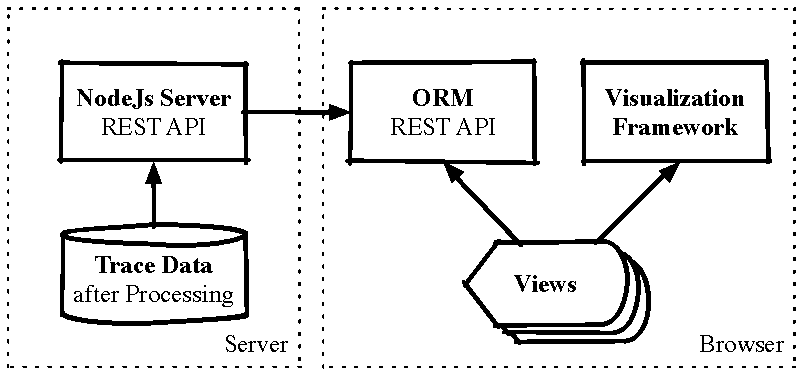
\includegraphics[width=\linewidth]{img/visualization_framework}
\caption{The visualization component of Parceive.}
\label{fig:visualization}
\end{figure}

\paragraph{Trace Optimization}
Parceive uses file-based databases to store trace data. Its
layout is optimized for writing to reduce the runtime overhead. All the
information required by the views can be obtained by using database queries.
However, most of the operations would take a disproportionate amount of time to
complete without applying trace optimization. This step is performed by
post-processing to dramatically reduce lookup times of views.   

Most importantly, the creation of selected indexes dramatically reduces lookup
times by allowing highly optimized search strategies. Since no additional data
will be added to the traces, creating redundancy generates no overhead and does
not increase the complexity. By adding additional fields and creating
intermediary tables, it is possible to avoid joins for most queries executed by
the visualizations. 

Executing \texttt{VACUUM} after all processing is done also improves
performance by reducing the fragmentation of data stored inside tables. The
increased locality of data reduces the execution time of most queries and has a
considerable effect on ones that require a full table scan. \texttt{VACUUM} is
also able to reduce the size of the processed
database.

\paragraph{On-Demand Loading}
The first service that improves responsiveness is on-demand loading of trace
data and its caching for reuse across views. Often, loading entire traces
into the browser is not possible due to memory restrictions. To solve this
problem a NodeJS server was developed that reads data from post-processed 
databases (see Section \ref{dataprocessing}) on demand. The server exposes a
REST \cite{rest} API that manages the retrieval of data. For security reasons
all SQL queries are contained in this server without supporting arbitrary
queries. The implementation makes use of multiple parallel reads to the same
database to reduce the latency and throughput when large amounts of data is
requested by the views. This service enables users to seamlessly navigate and
explore their software across multiple views.

The second service for a better scalability is abstraction of fine-grained
trace information to high-level entities. Examples are function invocations
that are grouped to call-groups, or runtime objects that lead to the
respective classes. 

Such abstractions are enabled by a Object Relational Mapper
(ORM) module to simplify development and improve performance. The ORM makes it
possible to access entities and to easily navigate the relationships
between them. The API is implemented using promises \cite{promises} simplifying
the asynchronous and parallel behavior. 

Such abstractions allow users to better comprehend their
software by using effective top-down approaches. 


The third service comprises a
communication infrastructure for
sharing arbitrary state across multiple views. This service can be used to spot
and restrict the current range of view to crucial points in the trace. Equipped
with all these services, the visualization framework allows scalable views for
software analysis.


\subsubsection*{Performance}

Figure \ref{parceive:procperformance} shows the time and size overhead of
processing databases generated by Parceive. The time required by this operation
is negligible because loading most visualizations without the optimizations
would waste more than the processing itself. The executed queries are also
heavily optimized making \texttt{VACUUM} and the creation of indexes the most
time consuming operations. The size increase is unfortunately unavoidable.

\begin{figure}
	\centering
	\begin{tabular}{l l l l}
		Database & Size & Processed Size & Time taken \\
		emsim\_par & 3905536 & 14560256 & 8.77 s
	\end{tabular}
	\caption{Database processing performance}
	\label{parceive:procperformance}
\end{figure}

\subsection{ORM}



The greatest benefit to using this ORM in visualizations is the possibility of
applying optimizations to the data loading. The most important ones are caching
and pipelining. Caching allows the ORM to avoid loading data that has been
accessed before. Each time an entity is retrieved from the server it is saved
and reused for subsequent requests. This optimization allows visualizations to
focus more on data presentation instead of efficient data retrieval.

Pipelining combines multiple queries to the same endpoint into a single one.
When requesting a large number of entities it can improve performance despite
the limit on the number of parallel requests in browsers. This optimization is
designed to greatly increase throughput at the cost of a response time
increased by 10 milliseconds.

\subsubsection{State management}

The visualization framework implements a centralized and persistent state
storage for visualizations. With the use of this feature it is possible to
retain the state of views across page loads.

Currently the view layout and the marked nodes are stored as part of the state
automatically. In addition to this each visualization can save tailored
information at any time and retrieve it when rendering. Local storage is used
to house all the state information making it persistent.

\subsubsection{Communication}

Visualizations perform different tasks and allow the user to navigate the
callgraph in different ways. Communication makes it possible to follow a chain
of investigation along multiple visualizations. Currently there are three ways
to communicate intent:

\begin{itemize}
	\item[Focus] brings entities to the attention of the user
	\item[Mark] allows the creation of selections that are visible between
visualizations
	\item[Spot] replaces all the entities in a visualization with a new set
	\item[Hover] brings entities to the attention of the user using opacity
\end{itemize}